\chapter{System Architecture}
\label{chap:ch3}

\par The architecture of this workforce management application was designed following modern, enterprise-grade software engineering principles. To ensure high cohesion, loose coupling, and horizontal scalability, the system adopts a decoupled Client-Server Architecture.

The application is strictly divided \textbf{into 4 distinct tiers}: a relational Data Persistence layer, a robust Application layer driven by an Inversion of Control (IoC) container, a secure stateless Integration layer, and a component-based Presentation layer. At the core of the Application layer sits a \textbf{custom heuristic solver}, designed specifically to address the complex \textbf{Constraint Satisfaction Problem (CSP) of generating Labor Code-compliant shift schedules}. By separating these concerns, the architecture ensures that the algorithmic complexity of the backend is entirely abstracted away from the end-user, resulting in a secure, responsive, and easily maintainable system.

\begin{figure}[!h]
    \centering
    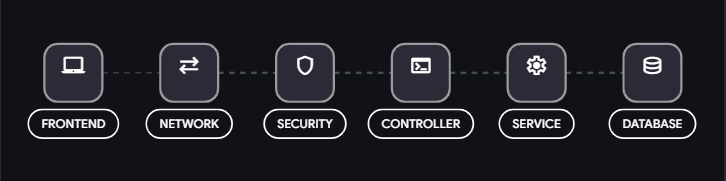
\includegraphics[width=1\linewidth]{Diagrama.png}
    \caption{Overview of data flow}
    \label{fig:dataFlow}
\end{figure}


\section{Technological Stack Overview}
\label{sec:ch3sec1}

\par The technological stack overview represents a comprehensive overview of the selected technological stack, detailing the rationale behind each architectural decision. Rather than relying on a tightly coupled monolithic structure, this system utilizes a modern, decentralized stack. Each framework and tool was deliberately chosen for its ability to fulfill specific architectural requirements, ranging from secure data persistence to complex algorithmic processing and dynamic user interaction.


\subsection{Data persistence : Microsoft SQL Server}
\label{subsec:ch3sec1subsec1}

\par For the underlying relational database tier, Microsoft SQL Server was selected. As a Tier-1 enterprise Relational Database Management System, it provides strict ACID (Atomicity, Consistency, Isolation, Durability) compliance, ensuring absolute data integrity for critical domain entities such as user credentials, store configurations, and generated labor shifts. Its seamless integration with SQL Server Management Studio (SSMS) also facilitates efficient database administration, querying, and schema verification during the application lifecycle. Moreover, the ability to easily integrate this DB with the best clouding hosts available (AWS and Microsoft Azure) makes it the best option available. \cite{pass2025}

\subsection{Application logic: Java + Spring Boot}
\label{subsec:ch3sec1subsec2}

\par The core backend logic, including the custom heuristic scheduling algorithm, is implemented using Java 17 and the Spring Boot 3 framework. Spring Boot was chosen primarily for its powerful Inversion of Control (IoC) container, which drastically reduces structural boilerplate and manages object lifecycles through Dependency Injection. It also provides the Spring Security module, which is broken down in the Security subsection. Furthermore, the integration of Spring Data JPA abstracts complex SQL queries into a highly efficient Object-Relational Mapping (ORM) layer via Hibernate, allowing the application layer to interact with the database efficiently and safely, while keeping the code clean and modern. Moreover, Java + Spring Boot is arguably the most used combination of tools worldwide for these types of application, therefore automatically granting multiple quality references and documents to learn and debug from, should there be any problems whatsoever.\cite{GuideOnJavaAndSpringBoot}

\subsection{Integration and security: REST and JWT}
\label{subsec:ch3sec1subsec3}

\par To ensure complete decoupling between client and server, communication is handled exclusively via a \textbf{RESTful API}. The API is secured with a stateless JWT-based pipeline in Spring Security, so the server does not keep session state in memory. On each request, the token is validated cryptographically to recover the user identity (subject), and the backend loads the user from the database via \texttt{UserDetailsService} to obtain the current roles/authorities for RBAC enforcement. This keeps the system stateless while still relying on per-request database lookups for user role resolution. In this design, role changes or user deactivation take effect immediately, because each request revalidates the user against the database before authorization is granted. \cite{mario2025hybrid}

\subsection{Presentation layer: React}
\label{subsec:ch3sec1subsec4}
\par The frontend presentation layer was developed using React, a component-based JavaScript library. React was selected specifically for its Virtual DOM architecture, which enables highly efficient, localized rendering of complex user interfaces. This is an essential requirement for this application, as rendering interactive, multi-dimensional monthly shift schedules requires rapid UI updates without reloading the entire web page. The component-driven approach also ensures high code reusability and maintainability across the application's administrative dashboards.

\begin{figure}[!h]
    \centering
    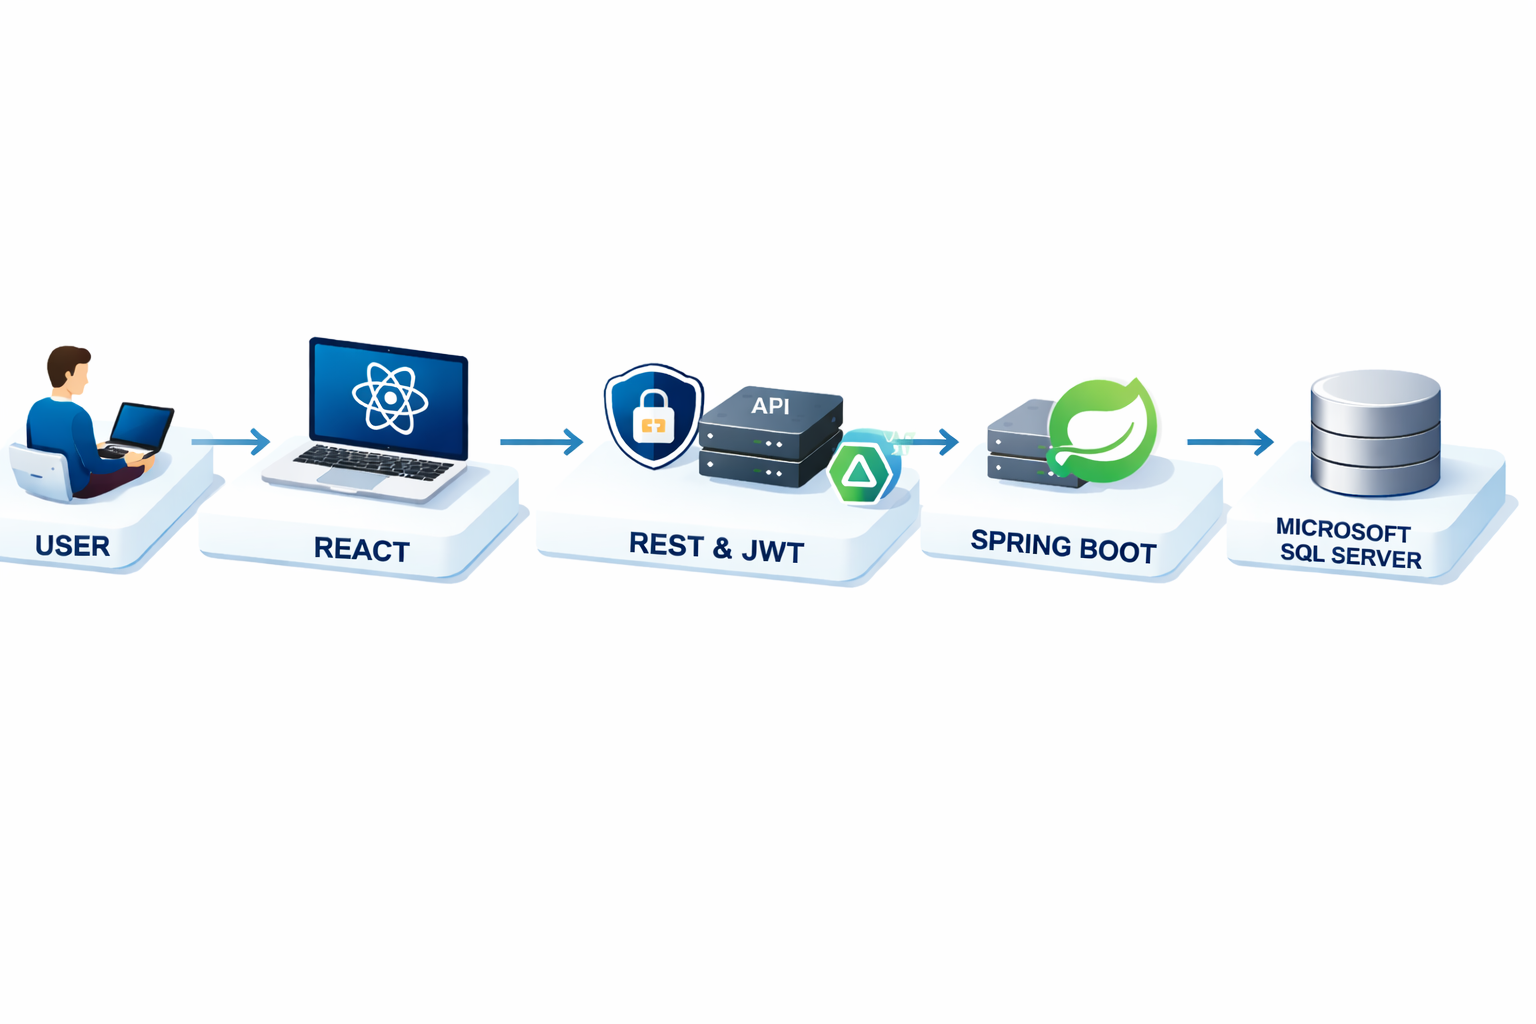
\includegraphics[width=1\linewidth]{DiagramTechStack.png}
    \caption{Technology Stack High Overview}
    \label{fig:tech_stack}
\end{figure}

\section{Practical Application of the System Architecture}
\label{sec:ch3sec2}

\par This section delves into the practical application of the technologies that form the backbone of the workforce management application. While the previous section justified the choice of each technology, this section focuses on their real-world implementation and interaction within the system.

\subsection{Database layer: Data integrity and accessibility}
\label{subsec:ch3sec2subsec1}

\par The database layer, implemented using Microsoft SQL Server, is structured to ensure data integrity and accessibility. Critical entities such as user credentials, labor shifts, and store configurations are stored in normalized tables to minimize redundancy and maintain consistency. The database schema is designed to enforce relationships and constraints, ensuring that the data remains reliable and secure.

\par The integration with Spring Data JPA allows the application layer to interact with the database through a high-level abstraction. This eliminates the need for manual SQL queries, as the ORM layer translates Java objects into database operations. For example, user registration and authentication processes involve creating and querying user records, which are seamlessly handled by the repository layer.

\subsection{Application layer: Business logic implementation}
\label{subsec:ch3sec2subsec2}

\par The application layer is the core of the system, where the business logic is implemented. Using Java 17 and Spring Boot 3, this layer manages operations such as user authentication, shift scheduling, and data validation. The custom heuristic scheduling algorithm, designed to solve the Constraint Satisfaction Problem (CSP), is implemented here to generate Labor Code-compliant shift schedules.

\par Dependency Injection, facilitated by Spring Boot's IoC container, ensures that components such as the `AuthenticationService` and `JwtService` are loosely coupled and easily testable. For instance, the `AuthenticationService` handles user registration and login by validating input, encoding passwords, and generating JWT tokens for secure communication.

\begin{figure}[H]
    \centering

    \begin{subfigure}{\linewidth}
        \centering
        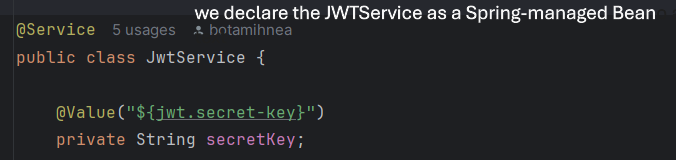
\includegraphics[width=0.65\linewidth,
                        height=0.10\textheight,
                        keepaspectratio]
                        {CodeSnippet-JwtService-Edit.PNG}
        \caption{JwtService Initialization}
    \end{subfigure}

    \vspace{0.2em}

    \begin{subfigure}{\linewidth}
        \centering
        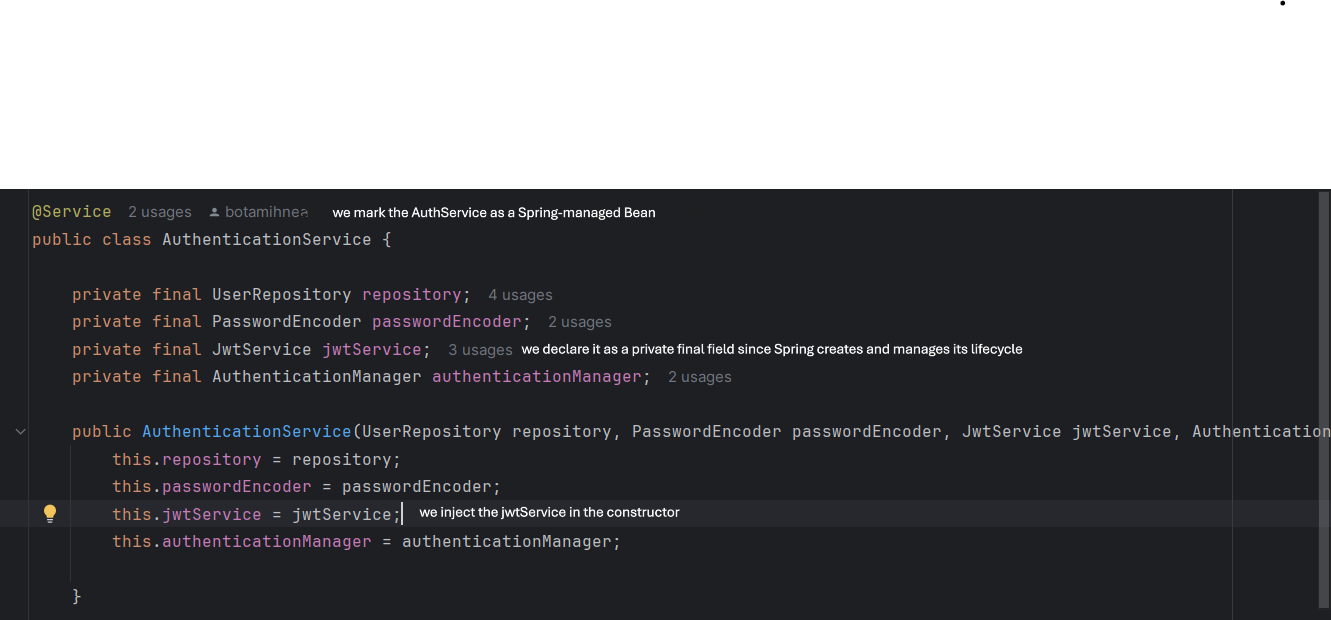
\includegraphics[
            width=0.80\linewidth,
            height=0.18\textheight,
            trim=20 20 20 20,
            clip]{CodeSnippet-AuthenticationService-Edited.PNG}
        \caption{AuthenticationService Initialization}
    \end{subfigure}

    \caption{Service initialization code snippets}
    \label{serviceInitCodeSnippets}
\end{figure}

\subsection{Integration layer: Secure communication}
\label{subsec:ch3sec2subsec3}

\par The secure bridge between the React frontend and the Spring Boot backend is facilitated by a custom Spring Security filter chain. Rather than relying on default session management, the system intercepts incoming HTTP requests using a custom \textbf{JwtAuthenticationFilter}.

\par When a client attempts to access a protected endpoint, such as the shift generation API, this filter extracts the Bearer token from the \textbf{Authorization} header. It then utilizes the \textbf{JwtService} to cryptographically verify the token's signature and expiration date. If valid, the user's role (e.g., \textbf{MANAGER}) is extracted from the database based on the user's identifier(email) from the token payload and injected into the \textbf{SecurityContextHolder}. This implementation allows the \textbf{SecurityConfig} class to seamlessly enforce Role-Based Access Control (RBAC) at the endpoint level, immediately rejecting unauthorized traffic with an HTTP 403 Forbidden status before it ever reaches the controller logic.

\subsection{Frontend layer: Dynamic user interaction}
\label{subsec:ch3sec2subsec4}

\par The frontend, developed using React, provides a dynamic and interactive user experience. By leveraging React's Virtual DOM, the application efficiently updates the user interface in response to user actions. For instance, when a user generates a shift schedule, the frontend sends a request to the backend API and updates the displayed schedule based on the response.

\par The component-based architecture of React ensures that the user interface is modular and maintainable. Each component is responsible for a specific part of the interface, such as the login form or the schedule viewer, making it easier to manage and extend the application.

\subsection{End-to-End workflow}
\label{subsec:ch3sec2subsec5}

\par The end-to-end workflow begins with the user interacting with the React-based frontend. User actions, such as submitting a login form, trigger HTTP requests to the backend API. The backend processes these requests by validating the JWT token, executing the necessary business logic, and interacting with the database as needed. The results are then returned to the frontend, which updates the user interface accordingly.

\par This workflow demonstrates the seamless integration of the chosen technologies, with each layer performing its role independently while contributing to the overall functionality of the system. By adhering to modern software engineering principles, the application achieves a balance between scalability and maintainability.


